% Setup -------------------------------

\documentclass[a4paper]{article}
\setcounter{secnumdepth}{3}
\setcounter{tocdepth}{3}

\usepackage{hyperref}
\usepackage{indentfirst}

\usepackage{graphicx}
\usepackage[export]{adjustbox}
\usepackage{float}

% Encoding
%--------------------------------------
\usepackage[T1]{fontenc}
\usepackage[utf8]{inputenc}
%--------------------------------------

% Portuguese-specific commands
%--------------------------------------
\usepackage[portuguese]{babel}
%--------------------------------------

% Hyphenation rules
%--------------------------------------
\usepackage{hyphenat}
%--------------------------------------

% References (BibTeX)
%--------------------------------------
\usepackage[backend=bibtex,style=numeric,sorting=ynt]{biblatex}
\usepackage[autostyle=true]{csquotes}
\addbibresource{Relatório.bib}
%--------------------------------------

% Capa do relatório

\title{
	Sistemas Distribuídos em Larga Escala
	\\ \Large{\textbf{Trabalho Prático}}
	\\ -
	\\ Mestrado em Engenharia Informática
	\\ Universidade do Minho
}
\author{
	\begin{tabular}{ll}
		\textbf{Grupo nº 1}
		\\
		\hline
		PG41080 & João Ribeiro Imperadeiro
        \\
		PG41081 & José Alberto Martins Boticas
		\\
        PG41091 & Nelson José Dias Teixeira
	\end{tabular}
}

\date{\today}

\begin{document}

\maketitle

% Introdução

\section{Introdução} \label{sec:Introduction}
\large{
	O presente relatório descreve o desenvolvimento do projeto de cariz prático da unidade curricular de Sistemas Distribuídos em Larga Escala.
	Neste trabalho é requerida a implementação de um dos algoritmos de agregação distribuída disponíveis na referência \parencite{article} indicada no enunciado do mesmo.
	Após concretizar a especificação do algoritmo escolhido, é posteriormente solicitado o teste do mesmo no simulador desenvolvido ao longo do semestre do presente ano letivo.

	Tal como é referido nos manuscritos \parencite{ref} e \parencite{article}, a agregação de dados distribuídos desempenha um papel bastante importante na concepção de diversos sistemas escaláveis uma vez que possibilita a determinação descentralizada de propriedades globais significativas, que posteriormente podem ser utilizadas para direcionar a execução de outras aplicações distribuídas.
	Vários algoritmos de agregação distribuída foram propostos ao longo dos últimos anos, exibindo propriedades diferentes em termos de precisão, desempenho e de comunicação. No entanto, muitas dessas abordagens não possuem caraterísticas relacionadas com a tolerância de falhas. Desta forma, no âmbito de sistemas distribuídos, este grupo de trabalho viu-se interessado em implementar um dos algoritmos associados a esta propriedade.

	Relativamente à estrutura deste relatório, é exibido o algoritmo escolhido pelos elementos deste grupo, apresentando o conceito e a implementação intrínsecos ao mesmo. Para além disso, são evidenciados alguns aspetos relativos ao simulador utilizado para proceder à realização de testes do algoritmo em causa, efetuando finalmente uma análise dos resultados obtidos.
}

\section{Algoritmo} \label{sec:Algorithm}
\large{
	Dos algoritmos de agregação distribuída presentes no documento referenciado no enunciado deste trabalho prático \parencite{article}, os elementos deste grupo optaram por escolher o algoritmo \textbf{\textit{flow updating}}.
	Este, ao nível de comunicação, é classificado como não estruturado, inserindo-se na categoria \textit{gossip} que, por sua vez, diz respeito à forma como as mensagens são disseminadas pela rede de comunicação.
	Quanto à perspetiva computacional, este algoritmo é baseado no conceito de \textit{averaging}, isto é, na computação iterativa de médias parciais que, ao longo do tempo, convergem para um resultado final previamente determinado.
	Esta última técnica permite também a derivação de outras funções de agregação (como por exemplo, \textit{count} ou \textit{sum}) de acordo com as combinações dos valores inicialmente instanciados.

	Uma das razões que levou este grupo a escolher este algoritmo foi a capacidade do mesmo em tolerar a injeção de falhas. Esta última caraterística é bastante importante sobretudo no que diz respeito à perda de mensagens trocadas na rede de comunicação.
	Para além desta vantagem associada ao contexto de sistemas distribuídos, este algoritmo possui não só um melhor desempenho quando comparado com os outros da mesma classe, como também possibilita uma computação precisa de valores.
	Por fim, a execução do algoritmo em causa é independente da topologia do roteamento de rede.

	No \hyperref[sec:Analysis of results]{4º capítulo} deste documento é apresentado todos os resultados obtidos após a implementação do algoritmo escolhido, discutindo-se a veracidade das propriedades mencionadas acima.

	\subsection{Conceito} \label{subsec:Concept}
	...

	\subsection{Implementação} \label{subsec:Implementation}
	...

	\begin{figure}[H]
		\centering
		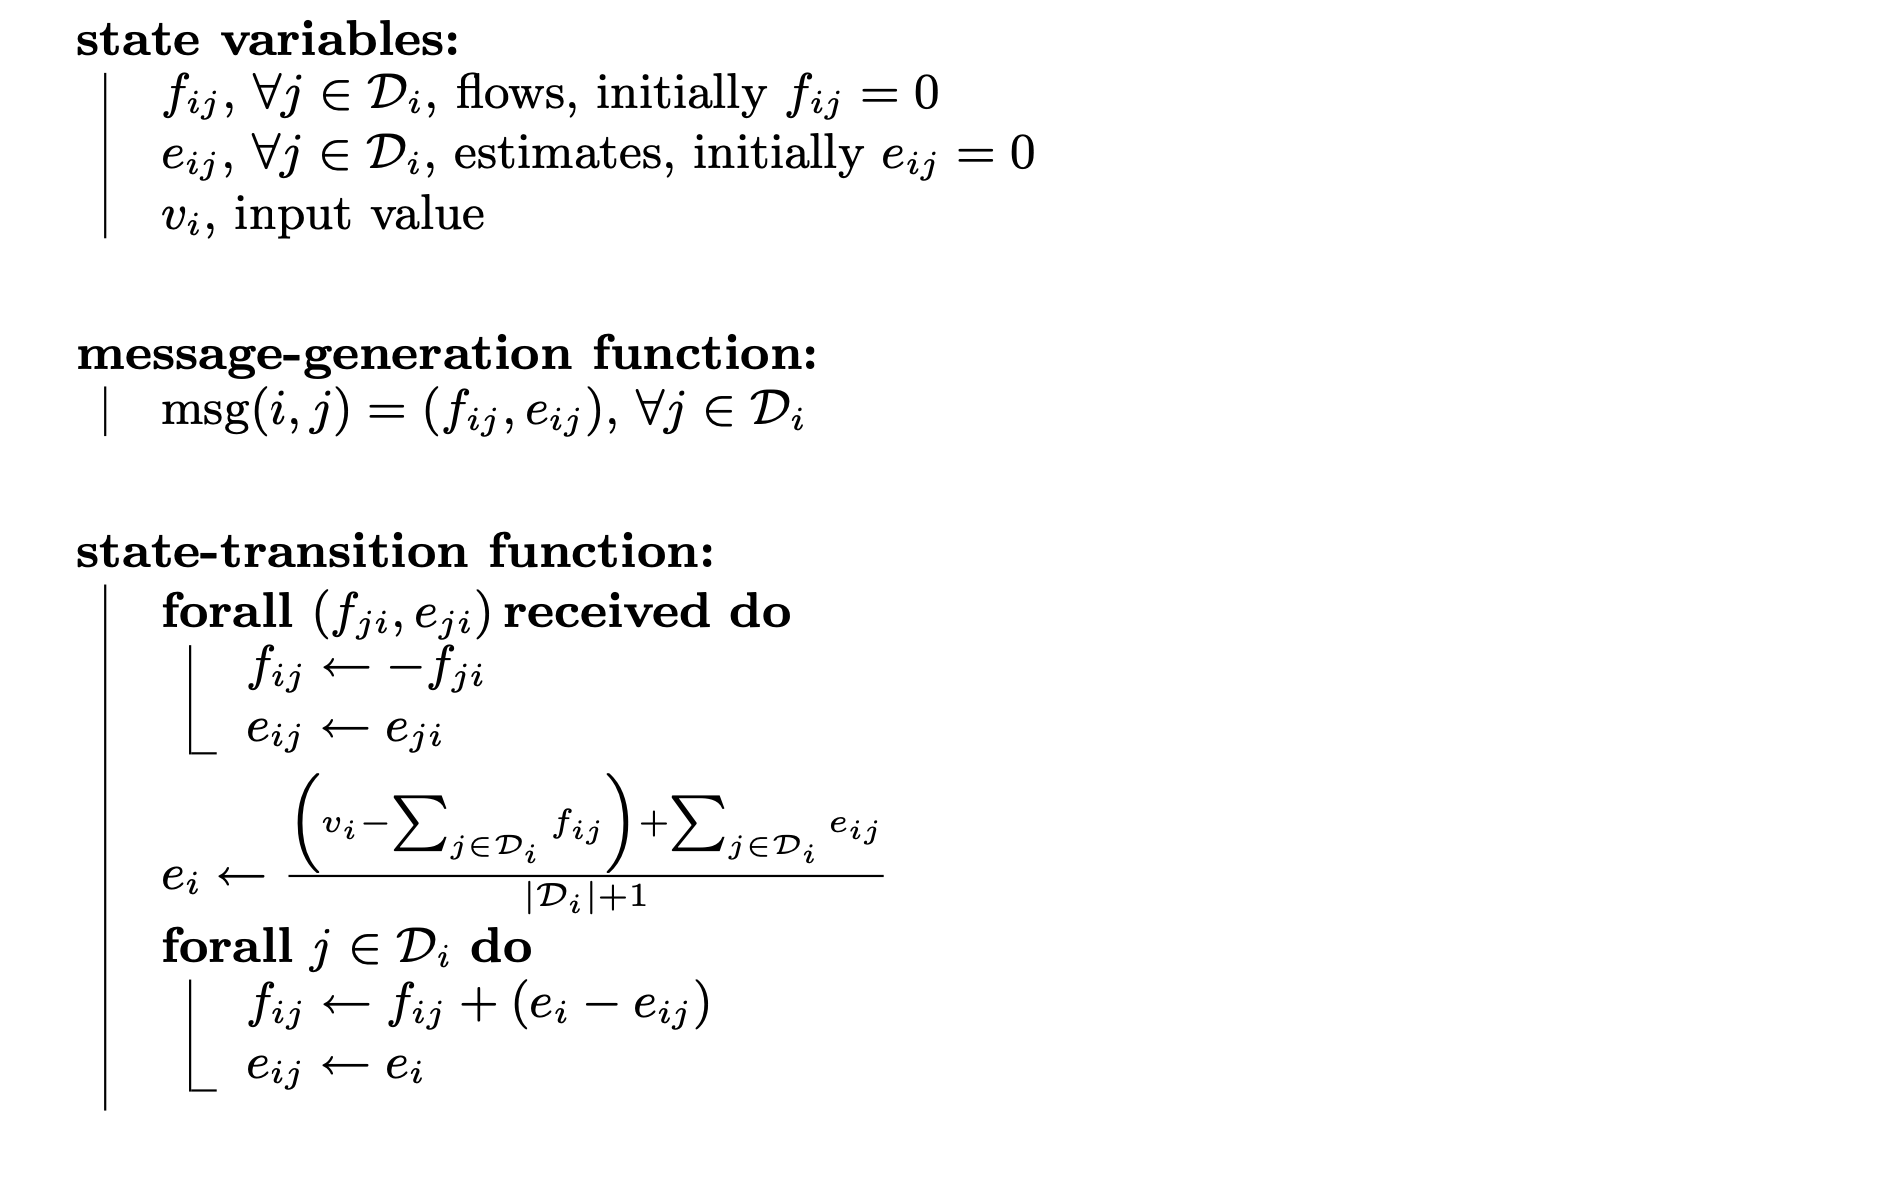
\includegraphics[width=1.0\textwidth, frame]{Imagens/Pseudocode.png}
		\caption{Pseudocódigo do algoritmo \textit{Flow Updating}}
		\label{fig:1}
	\end{figure}
}

\section{Simulador} \label{sec:Simulator}
\large{
	...
}

\section{Análise de resultados obtidos} \label{sec:Analysis of results}
\large{
	...
}

\section{Conclusão} \label{sec:Conclusion}
\large{
	...
}

\printbibliography[heading=bibintoc]

\end{document}